\section{Stable Graphs} \label{sec:section_3}

    In this section we introduce the class of \emph{stable} graphs.
    A graph is considered stable, if it does not contain bi-induced (as defined in~\cite{induced_subgraph_density_vi_bounded_vc_dimension})
    \todo{Maybe move cite to section 2, and mention there other references such as "induced sub-bigraph"}
    large half-graphs, a particularly \irregular\todo{Explain somewhere what this means.}~structure in graphs.
    See \Cref{fig:half-graph} for an example of such a graph.

    \begin{figure}
    \centering

    % Parameters
    \def\nodessep{1}
    \def\n{10} % Number of nodes (each part)
    \def\cellsize{0.5} %set as 5 divided by \n

    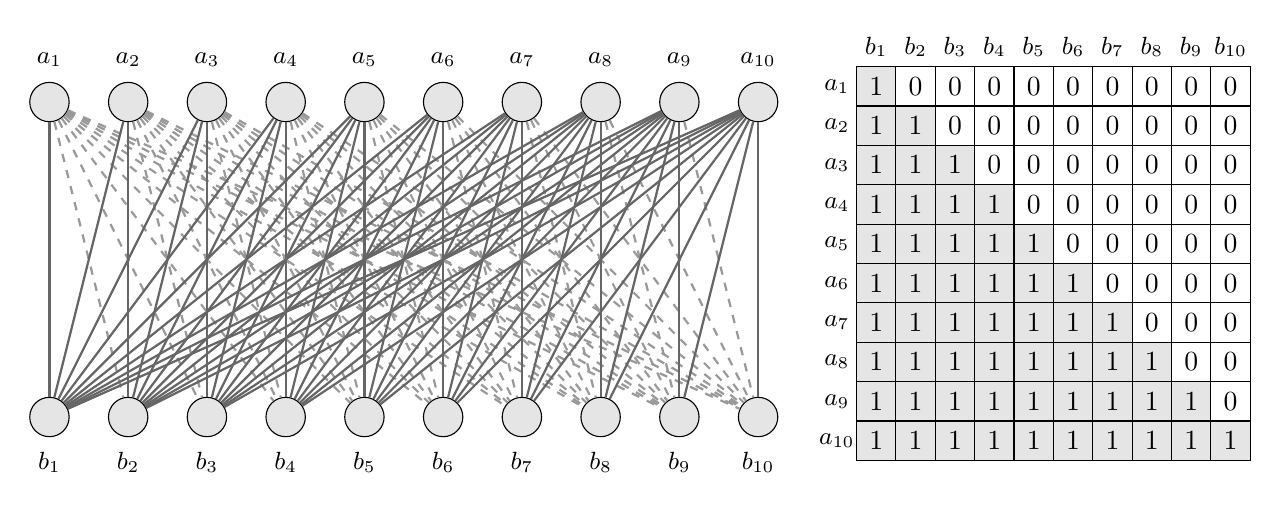
\begin{tikzpicture}[
        vertex/.style={circle, draw, fill=gray!20, minimum size=5mm, inner sep=1pt},
        label_a/.style={above=2pt, font=\small},
        label_b/.style={below=2pt, font=\small},
        node distance=1.5cm,
        solid edge/.style={draw, thick, black!60},
        dashed edge/.style={draw, dashed, thick, black!40},
        matrix cell/.style={draw, minimum size=\cellsize cm, inner sep=0pt},
        matrix label/.style={font=\small, anchor=center}
    ]

    % Graph nodes (top and bottom)
    % Top part vertices (a_i)
    \foreach \i in {1,...,\n} {
        \node[vertex] (a\i) at (\i*\nodessep, 0) {};
        \node[label_a] at (a\i.north) {$a_{\i}$};
    }

    % Bottom part vertices (b_j)
    \foreach \j in {1,...,\n} {
        \node[vertex] (b\j) at (\j*\nodessep, -4) {};
        \node[label_b] at (b\j.south) {$b_{\j}$};
    }

    % Draw edges
    \foreach \i in {1,...,\n} {
        \foreach \j in {1,...,\n} {
            \ifnum\i<\j
                \draw[dashed edge] (a\i) -- (b\j);
            \else
                \draw[solid edge] (a\i) -- (b\j);
            \fi
        }
    }

    % Adjacency Matrix
    \begin{scope}[xshift=2cm+\n*\nodessep cm]

    % Matrix labels
    \foreach \i in {1,...,\n} {
        \node[matrix label] at (-1 + \i*\cellsize, 0.7) {$b_{\i}$};
        \node[matrix label] at (-1, 0.7 -\i*\cellsize) {$a_{\i}$};
    }

    % Draw the matrix cells and fill based on adjacency
    \foreach \i in {1,...,\n} {
        \foreach \j in {1,...,\n} {
            \pgfmathsetmacro{\xcoord}{\j*\cellsize}
            \pgfmathsetmacro{\ycoord}{-\i*\cellsize}
            \ifnum\i<\j
                \node[matrix cell] at (-1 + \xcoord, 0.7 + \ycoord) {0};
            \else
                \node[matrix cell, fill=gray!20] at (-1 + \xcoord, 0.7 + \ycoord) {1};
            \fi
        }
    }

    \end{scope}

    \end{tikzpicture}
    \caption{
        A half-graph with 2 × 10 vertices.
        \emph{On the left}, solid lines show adjacent vertices, and dashed lines show non-adjacent vertices.
        Pairs of vertices without a line may or may not be connected.
        \emph{On the right} is the corresponding adjacency matrix.
    }
    \label{fig:half_graph}
\end{figure}

    First, stability implies a bounded \emph{Vapnik-Chervonenkis (VC) dimension}, which limits the variety of
    neighborhoods of vertices within the graph.
    While stability implies a bounded VC-dimension for the entire graph
    (See~\cite{regularity_partitions_and_the_topology_of_graphons}), our work primarily focuses on bounding
    the VC-dimension restricted to a subset of vertices.
    This is formalized in \Cref{lem:k_order_property_bounds_BAbs}.

    Second, stability implies a finite \emph{tree bound}.
    This property is the foundational tool we use to prove the existence of parts that are \regular~with
    respect to the rest of the graph.
    We use this to establish the existence of indivisible parts in \Cref{sec:section_4}
    (\Cref{lem:existance_of_indivisible_sets}) and
    excellent parts in \Cref{sec:section_5} (\Cref{lem:existance_of_excellent_subsets}).

    \subsection{$k$-order Property} \label{subsec:subsection_3.1}

        First, we formally define stability as the non-$k$-order property, where $k$ determines the size of the
        excluded half-graphs.

        \begin{definition} \label{def:k_order_property}
            Let $G$ be a graph.
            We say that $G$ has the \emph{$k$-order property} if there exist two sequences of vertices
            $\Partriangle{a_i \mid i \in \parcurly{1, \dots, k}}$ and $\Partriangle{b_i \mid i \in \parcurly{1, \dots, k}}$ such that
            for all $i,j \leq k$, $a_i R b_j$ if and only if $i \geq j$.
            Otherwise, we say that $G$ has the \emph{non-$k$-order property} or that $G$ is \emph{$k$-stable}.
        \end{definition}

        \begin{remark}
            It is important to note what is left unspecified in \Cref{def:k_order_property}.
            First, the vertices within each sequence must be distinct, as their neighborhoods within the other sequence
            differ.
            However, the sequences themselves need not be disjoint.
            One may have $a_i=b_j$, provided $i < j$ (so that $\neg(a_i R b_j)$).
            Furthermore, the definition does not specify the presence or absence of edges within the same sequence.
            Consequently, the non-$k$-order property requires the containment of a subgraph from a broad class of structures,
            not merely a k-half-graph.
            \todo{Possibly add visual example of this too.}
        \end{remark}

        \begin{remark}
            $G$ having the $k$-order property implies that $G$ has the $k'$-order property for all $k' \leq k$.
            Conversely, $G$ having the non-$k$-order property implies that $G$ has the non-$k'$-order property for all $k' \geq k$.
        \end{remark}

        An important concept used all over the thesis is that of \emph{exceptional edges} and \emph{exceptional vertices}.
        That is, edges and vertices that, in the context of a pair of sets of vertices, do not \say{behave} as the rest.
        \todo{Echarle un ojo.}
        In order to classify what is the expected behaviour in a graph, or more specifically, in a pair of sets of vertices,
        we define the \emph{truth value}.

        \begin{definition}[Truth value] \label{def:truth_value}
            Let $G$ be a graph.
            For any (not necessarily disjoint) $A, B \subseteq G$, we say that
            \[
                t(A,B) =
                \begin{cases}
                    0 & \text{if } \parstraight{\parcurly{\parround{a, b} \in A \times B \mid a R b, a \neq b}} <
                        \parstraight{\parcurly{\parround{a, b} \in A \times B \mid \neg a R b, a \neq b}} \\
                    1 & \text{otherwise}
                \end{cases}
            \]
            is the \emph{truth value} of the pair $\parround{A,B}$.
            That is, $t(A,B) = 0$ if $A$ and $B$ are mostly disconnected, and $t(A,B) = 1$ if they are mostly connected.
            When $B = \parcurly{b}$, we write $t(A,b)$ instead of $t(A,\parcurly{b})$, and we say that it is the truth value of $A$
            with respect to $b$.
        \end{definition}

        In this context, we say that a vertex $a \in A$ is \emph{exceptional} with respect to $B \subseteq G$ if $t(a,B) \not\equiv t(A,B)$,
        or that it is exceptional with respect to $b \in G$ if $a R b \not\equiv t(A,b)$.
        On the other hand, we say that an edge $ab$ with $a \in A$ and $b \in B$ is exceptional in $(A,B)$ if $a R b \not\equiv t(A,B)$.
        Also, it is useful to define the following set of vertices.
        \begin{itemize}
            \item $B_{A,b} = \parcurly{a \in A \mid a R b \equiv t(A,b)}$, i.e. the set of non-exceptional vertices of $A$
                with respect to $B$.
            \item $\overline{B}_{A,b} = \parcurly{a \in A \mid a R b \not\equiv t(A,b)}$, the set of exceptional vertices of $A$ with
                respect to $B$.
            \item $B^+_{A,b} = \parcurly{a \in A \mid a R b}$, the vertices of $A$ connected to $b$.
            \item $B^-_{A,b} = \parcurly{a \in A \mid \neg a R b}$, the vertices of $A$ that are not connected to $b$.
        \end{itemize}
        With this notation, notice that either $t(A,b) = 1$ and thus $B_{A,b} = B^+_{A,b}$, or $t(A,b) = 0$ and $B_{A,b} = B^-_{A,b}$.

        Sets of vertices $A$ with a large number of large $\overline{B}_{A,b}$ are a great obstacle towards creating a \regular,
        and more specifically homogeneous \todo{Define homogeneous} partition, as the number of exceptional edges with respect
        to the entire graph is large and concentrated.
        A useful tool to deal with them is \Cref{lem:k_order_property_bounds_BAbs}, which gives a bound on the number of
        such sets under the non-$k$-order property.
        In order to prove it, we first need to introduce the \emph{VC dimension} of a family of sets, and relate it to the
        $k$-order property.
        This, together with \Cref{lem:sauer-shelah}, will give us the desired result.

        \begin{definition} \label{def:shattered}
            Let $G$ be a set and $S = \parcurly{S_i \subseteq G \mid i \in I}$ be a family of sets.
            A set $A \subseteq G$ is said to be \emph{shattered} by $S$ (and $S$ is said to \emph{shatter} $A$) if
            for every $B \subseteq A$, there exists $S_i \in S$ such that $S_i \cap A = B$.
        \end{definition}

        \begin{definition} \label{def:VC_dimension}
            Let $G$ be a set and $S = \parcurly{S_i \subseteq G \mid i \in I}$ be a family of sets.
            The \emph{VC dimension} of $S$ is the size of the largest set $A \subseteq G$ that is shattered by $S$.
        \end{definition}

        \begin{lemma}[Sauer-Shelah (-Perles -Vapnik-Chervonenkis) Lemma,
                \cite{on_the_density_of_families_of_sets},
                \cite{a_combinatorial_problem_stability_and_order_for_models_and_theories_in_infinitary_languages}]
            % 4 names with parenthesis title from: https://gilkalai.wordpress.com/2008/09/28/extremal-combinatorics-iii-some-basic-theorems/
            \label{lem:sauer-shelah}  % both authors proved this independently
            Let $G$ be a set and $S = \parcurly{S_i \subseteq G \mid i \in I}$ be a family of sets.
            If the VC dimension of $S$ is at most $k$, and the union of all the sets in $S$ has $n$ elements, then
            $S$ consists of at most $\sum_{i=0}^{k} \binom{n}{i} \leq n^k$ sets.
        \end{lemma}

        We'll begin by proving a stronger version of this lemma from Pajor, for which Sauer-Shelah will be a straightforward
        consequence.

        \begin{lemma}[Pajor's variant,~\cite{sous_spaces_1_des_espaces_de_banach_travaux_en_cours}] \label{lem:pajor}
            Let $G$ be a set and $S$ be a finite family of sets in $G$.
            Then $S$ shatters at least $\parstraight{S}$ sets.
            \begin{proof}
                We will prove this by induction on the cardinality of $S$.
                If $\parstraight{S} = 1$, then $S$ consists of a single set, which only shatters the empty set.
                If $\parstraight{S} > 1$, we may choose an element $x \in S$ such that some sets of $S$ contain $x$ and some do not.
                Let $S^+ = \parcurly{s \in S \mid x \in S}$ and $S^- = \parcurly{s \in S \mid x \not\in S}$.
                Then $S = S^+ \sqcup S^-$, and both $S^+$ and $S^-$ are non-empty.
                By induction hypothesis, we know that $S^+ \subsetneq S$ shatters at least $\parstraight{S^+}$ sets,
                and $S^- \subsetneq S$ shatters at least $\parstraight{S^-}$ sets.
                Let $T, T^+, T^-$ be the families of sets shattered by $S$, $S^+$ and $S^-$ respectively.
                To conclude the proof, we just need to show that for each element in $T^+$ and $T^-$, there is a corresponding
                one in $T$.
                If a set is shattered by only one of the two families $S^+$ and $S^-$, then it only contributes by one unit
                to $\parstraight{T^+} + \parstraight{T^-}$ and one unit to $\parstraight{T}$.
                Notice that no set shattered by $S^+$ or $S^-$ may contain $x$, otherwise all or none of the intersections
                will contain this element.
                Thus, if a set $s$ is shattered by both $S^+$ and $S^-$, it will contribute by two units to
                $\parstraight{T^+} + \parstraight{T^-}$ and one unit to $\parstraight{T}$.
                But then, for each such set, we can consider $s \cup \parcurly{x}$ which is not in $T^+$ or $T^-$, but it is in $T$.
                Indeed, for each subset of $s$, if it does not contain $x$ it is the intersection with some
                set in $S^- \subsetneq S$, and if it does contain $x$ it is the intersection with some set in $S^+ \subsetneq S$.
                All in all, we conclude that
                \[
                    \parstraight{T} \geq \parstraight{T^+} + \parstraight{T^-} \geq \parstraight{S^+} + \parstraight{S^-}
                                    \geq \parstraight{S}
                \]
            \end{proof}
        \end{lemma}

        \begin{proof}[Proof of \Cref{lem:sauer-shelah}.]
            Suppose that $\bigcup S$ has $n$ elements.
            By \Cref{lem:pajor}, $S$ shatters at least $\parstraight{S}$ subsets, and since there are at most
            $\sum_{i=0}^k \binom{n}{i}$ subsets of $S$ of size at most $k$, if
            $\parstraight{S} > \sum_{i=0}^k \binom{n}{i}$, at least one of the shattered sets has cardinality larger than $k$,
            and hence the VC dimension of $S$ is larger than $k$.
        \end{proof}

        Next, we want to prove that if $G$ has the non-$k$-order property, then the size of the family of exceptional
        sets of $A$, relative to each vertex $b \in G$, is bounded by $|A|^k$.
        Instead, we prove a stronger result, that is we prove this same bound with only the condition that $G$
        has the \say{disjoint} non-$k$-order property, in which the two sequences of vertices in the \Cref{def:k_order_property}
        are in fact disjoint.
        This stronger version (\Cref{lem:k_order_property_bounds_BAbs}) is neither more useful nor easier to prove,
        but remarks that the non-disjointness of the sequences, and thus the broadening of the excluded structures,
        is not needed to obtain the bound, but later on.

        \begin{lemma} \label{lem:vc_dimension_implies_k_order_property}
            Let $G$ be a graph and $A \subseteq G$.
            Let $S = \parcurly{B^+_{A,b} \mid b \in G \setminus A}$.
            If $S$ has VC dimension (at least) $k$, then $G$ has the (disjoint)
            \todo{Lluis: faig una definició separada o s'enten pel context que ja he posat?}
            $k$-order property.
            \begin{proof}
                If $S$ has VC dimension $k$, then it shatters a set $A' \subseteq A$ of size $k$.
                Now, choose any order of the vertices of $A' = \Partriangle{a_1, \dots, a_k}$.
                Then, consider the increasing sequence of subsets $A_1 \subseteq A_2 \subseteq \dots \subseteq A_k = A'$,
                where $A_i = \parcurly{a_j \mid j \in \parcurly{1, \dots, i}}$.
                Since $A'$ is shattered by $S$, for each $i \in \parcurly{1, \dots, k}$ there exists a $b_i \in G$ such that
                $b_i R a$ if and only if $a \in A_i$.
                In particular, the two sequences $\Partriangle{a_i \mid i \in \parcurly{1, \dots, k}}$ and
                $\Partriangle{b_i \mid i \in \parcurly{1, \dots, k}}$ satisfy
                \[
                    a_i R b_j \Leftrightarrow i \leq j
                \]
                and thus $G$ has the $k$-order property.
            \end{proof}
        \end{lemma}

        \begin{lemma}[Claim 2.6 in~\cite{regularity_lemmas_for_stable_graphs}] \label{lem:k_order_property_bounds_BAbs}
            Let $G$ be a graph with the (disjoint) non-$k$-order property.
            Then, for any finite non-trivial $A \subseteq G$,
            \[
                \parstraight{\parcurly{B^+_{A,b} \mid b \in G}} \leq |A|^k
            \]
            \begin{proof}
                By \Cref{lem:vc_dimension_implies_k_order_property}, if $G$ has the non-$k$-order property,
                then the family $\parcurly{B^+_{A,b} \mid b \in G \setminus A}$ has VC dimension at most $k-1$,
                so by the Sauer-Shelah \Cref{lem:sauer-shelah} we have
                $\parcurly{B^+_{A,b} \mid b \in G \setminus A} \leq \sum_{i=0}^{k-1} \binom{|A|}{i}$.
                Since $\parcurly{B^+_{A,b} \mid b \in A} \leq \parstraight{A}$, we conclude that
                \[
                    \parstraight{S} = \parstraight{\parcurly{B^+_{A,b} \mid b \in G}} \leq \sum_{i=0}^{k-1} \binom{|A|}{i} + |A|
                \]
                Finally, when $\parstraight{A} = n,k > 1$: \todo{This conditions should be set at some point of the tfm. Specify that if they are not met, the problem becomes trivial.}
                \begin{itemize}
                    \item if $n \leq k$, then $\parstraight{S} \leq 2^n \leq 2^k \leq n^k$.
                    \item if $n > k$, then $\parstraight{S} \leq \sum_{i=0}^{k-1} {n \choose i} + n \leq n^{k-1} + n \leq 2n^{k-1} \leq n^k$.
                \end{itemize}
                We conclude that $\parstraight{S} \leq n^k$.
            \end{proof}
        \end{lemma}

        \begin{remark}
            The condition $n,k > 1$ is trivial.
            If $n=1$ then $A$ is the trivial graph with a single vertex.
            If $k=1$ we are not allowing even a single edge, so $G$ is the empty graph.
        \end{remark}

        We now prove the following equivalent versions of the lemma, which will be useful in the different sections of the
        thesis.
        The idea is that any choice of either the exceptional or the non-exceptional vertices set of $A$ with respect to
        each vertex $b \in G$, have the same bound.

        \begin{corollary}[Claim 2.6.1] \label{cor:k_order_propery_bounds_BAbs}
            Let $G$ be a graph with the non-$k$-order property.
            Then:
            \begin{enumerate}
                \item\label{itm:k_order_propery_bounds_BAbs.1} For any finite $A \subseteq G$
                    \[
                        \parstraight{\parcurly{B^-_{A,b} \mid b \in G}}
                            \leq |A|^k
                    \]
                \item\label{itm:k_order_propery_bounds_BAbs.2} For any finite $A \subseteq G$
                    \[
                        \parstraight{\parcurly{\overline{B}_{A,b} \mid b \in G}}
                            \leq |A|^k
                    \]
            \end{enumerate}
            \begin{proof}
                \begin{enumerate}
                    \item First of all, notice that $B^+_{A,b} = A - B^-_{A,b}$, since by definition they are complementary.
                        Thus, for any $b, b' \in G$, $B^+_{A,b} = B^+_{A,b'} \Leftrightarrow B^-_{A,b} = B^-_{A,b'}$.
                        It follows that
                        \[
                            \parstraight{\parcurly{B^-_{A,b} \mid b \in G}} =
                            \parstraight{\parcurly{B^+_{A,b} \mid b \in G}} \leq |A|^k
                        \]
                        where the last inequality follows from \Cref{lem:k_order_property_bounds_BAbs}.
                    \item Consider the following map:
                        \begin{align*}
                            \pi: \parcurly{B^+_{A,b} \mid b \in G} & \longrightarrow \parcurly{\overline{B}_{A,b} \mid b \in G} \\
                                                         B^+_{A,b} & \longmapsto \overline{B}_{A,b}
                        \end{align*}
                        We first prove that the map $\pi$ is well-defined.
                        If $B^+_{A,b}$ and $B^+_{A,b'}$ are equal, then they have the same size, and thus the same truth value.
                        Then,
                        \begin{itemize}
                            \item if $t(A,b) = t(A,b') = 1$, we have that $\overline{B}_{A,b} = B^+_{A,b} = B^+_{A,b'} = \overline{B}_{A,b'}$.
                            \item if $t(A,b) = t(A,b') = 0$, we have that
                            $\overline{B}_{A,b} = B^-_{A,b} = A \setminus B^+_{A,b} = A \setminus B^+_{A,b'} = B^-_{A,b'} = \overline{B}_{A,b'}$.
                        \end{itemize}
                        which proves that the map is well-defined.
                        The map $\pi$ is also surjective, since for each $b \in G$, and thus for each $\overline{B}_{A,b}$,
                        the set $B^+_{A,b}$ is mapped to $\overline{B}_{A,b}$ by construction.
                        Hence,
                        \[
                            \parstraight{\parcurly{\overline{B}_{A,b} \mid b \in G}} \leq
                            \parstraight{\parcurly{B^+_{A,b} \mid b \in G}} \leq
                            \sum_{i \leq k} \binom{|A|}{i} \leq |A|^k
                        \]
                        This concludes the proof.
                        Notice that, actually, the map $\pi$ is a not necessarily a bijection, since (at most) two $b$'s with
                        different truth value with respect to $A$ may induce the same set $\overline{B}_{A,b}$.
                \end{enumerate}
            \end{proof}
        \end{corollary}

    \subsection{Tree Bound} \label{subsec:subsection_3.2}

        During the next sections, it will be a key point proving that some sort of \say{regular} subgraphs
        (\emph{independent} in \Cref{sec:section_4} and \emph{excellent} in \Cref{sec:section_5}) exist in a given
        stable graph.
        In order to do so, a useful structure strongly related to the $k$-order property is the \emph{$k$-tree}.

        \begin{definition} \label{def:k-tree}
            A \emph{$k$-tree} in $G$ is an ordered pair $H = (\overline{c},\overline{b})$ comprising:
            \begin{itemize}
                \item $\overline{c} = \parcurly{ c_\eta \in G \mid \eta \in \parcurly{0,1}^{<k_{**}} }$, the set of \emph{nodes}.
                \item $\overline{b} = \parcurly{ b_\rho \in G \mid \rho \in \parcurly{0,1}^{k_{**}} }$, the set of \emph{branches}.
            \end{itemize}
            satisfying that, for all $\eta \in \parcurly{0,1}^{<k_{**}}$ and $\rho \in \parcurly{0,1}^{k_{**}}$,
            if given $\ell \in \parcurly{0, 1}$ we have $\eta \frown \Partriangle{\ell} \triangleleft \rho$, then
            $\parround{b_\rho R c_\eta} \equiv \parround{\ell = 1}$.
            The two sequences are not necessarily disjoint. \todo{Lluis: millor una remark?}
        \end{definition}

        See \Cref{fig:k_tree} for an example of such a structure.

        \begin{figure}
    \centering
    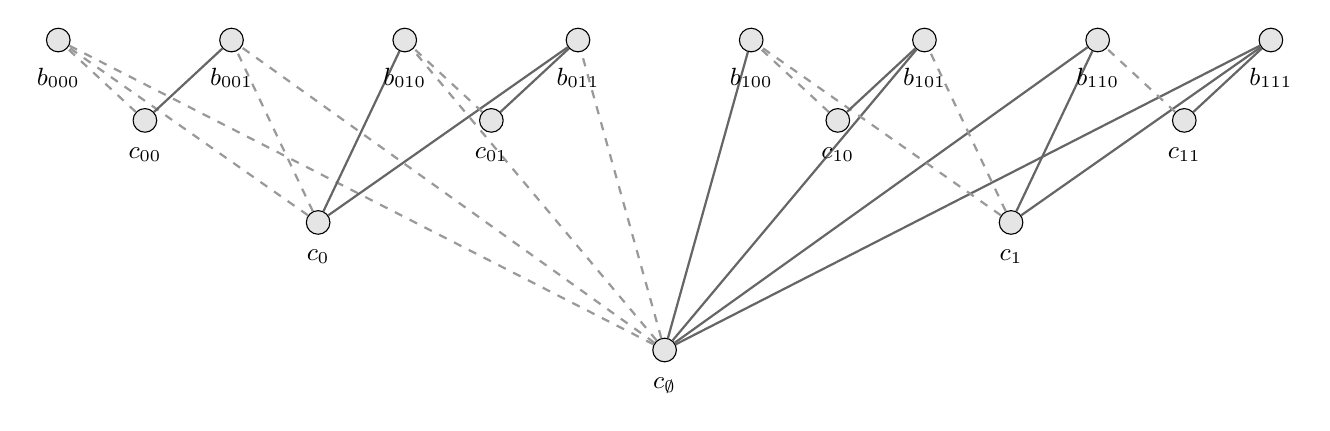
\begin{tikzpicture}[
        vertex/.style={circle, draw, fill=gray!20, minimum size=0.3cm, inner sep=1pt},
        label/.style={below=2pt, font=\small},
        solid edge/.style={draw, thick, black!60},
        dashed edge/.style={draw, dashed, thick, black!40},
    ]
	\node[vertex] (c_) at (8.8,0.0) {};
	\node[vertex] (c_0) at (4.4,1.62) {};
	\node[vertex] (c_1) at (13.200000000000001,1.62) {};
	\node[vertex] (c_00) at (2.2,2.9160000000000004) {};
	\node[vertex] (c_01) at (6.6000000000000005,2.9160000000000004) {};
	\node[vertex] (c_10) at (11.0,2.9160000000000004) {};
	\node[vertex] (c_11) at (15.400000000000002,2.9160000000000004) {};
	\node[vertex] (b_000) at (1.1,3.9366000000000008) {};
	\node[vertex] (b_001) at (3.3000000000000003,3.9366000000000008) {};
	\node[vertex] (b_010) at (5.5,3.9366000000000008) {};
	\node[vertex] (b_011) at (7.700000000000001,3.9366000000000008) {};
	\node[vertex] (b_100) at (9.9,3.9366000000000008) {};
	\node[vertex] (b_101) at (12.100000000000001,3.9366000000000008) {};
	\node[vertex] (b_110) at (14.3,3.9366000000000008) {};
	\node[vertex] (b_111) at (16.5,3.9366000000000008) {};
	\draw[dashed edge] (c_) -- (b_000);
	\draw[dashed edge] (c_) -- (b_001);
	\draw[dashed edge] (c_) -- (b_010);
	\draw[dashed edge] (c_) -- (b_011);
	\draw[solid edge] (c_) -- (b_100);
	\draw[solid edge] (c_) -- (b_101);
	\draw[solid edge] (c_) -- (b_110);
	\draw[solid edge] (c_) -- (b_111);
	\draw[dashed edge] (c_0) -- (b_000);
	\draw[dashed edge] (c_0) -- (b_001);
	\draw[solid edge] (c_0) -- (b_010);
	\draw[solid edge] (c_0) -- (b_011);
	\draw[dashed edge] (c_1) -- (b_100);
	\draw[dashed edge] (c_1) -- (b_101);
	\draw[solid edge] (c_1) -- (b_110);
	\draw[solid edge] (c_1) -- (b_111);
	\draw[dashed edge] (c_00) -- (b_000);
	\draw[solid edge] (c_00) -- (b_001);
	\draw[dashed edge] (c_01) -- (b_010);
	\draw[solid edge] (c_01) -- (b_011);
	\draw[dashed edge] (c_10) -- (b_100);
	\draw[solid edge] (c_10) -- (b_101);
	\draw[dashed edge] (c_11) -- (b_110);
	\draw[solid edge] (c_11) -- (b_111);
	\node[label] at (c_.south) {$c_{\emptyset}$};
	\node[label] at (c_0.south) {$c_{0}$};
	\node[label] at (c_1.south) {$c_{1}$};
	\node[label] at (c_00.south) {$c_{00}$};
	\node[label] at (c_01.south) {$c_{01}$};
	\node[label] at (c_10.south) {$c_{10}$};
	\node[label] at (c_11.south) {$c_{11}$};
	\node[label] at (b_000.south) {$b_{000}$};
	\node[label] at (b_001.south) {$b_{001}$};
	\node[label] at (b_010.south) {$b_{010}$};
	\node[label] at (b_011.south) {$b_{011}$};
	\node[label] at (b_100.south) {$b_{100}$};
	\node[label] at (b_101.south) {$b_{101}$};
	\node[label] at (b_110.south) {$b_{110}$};
	\node[label] at (b_111.south) {$b_{111}$};
    \end{tikzpicture}
    \caption{Example of a 3-tree. 
Notice that connections between disjoint sub-trees are not defined, and may be edges or non-edges in 
any combination.}
    \label{fig:k_tree}
\end{figure}


        Similarly to stability, we can define the \emph{tree bound} of a graph to measure the level of freeness from $k$-trees
        of graph.

        \begin{definition}[Definition 2.11] \label{def:tree_bound}
            Suppose $G$ is a finite graph.
            We denote the \emph{tree bound} $k_{**} = k_{**}(G)$ as the minimal positive integer such that there is no
            $k_{**}$-tree $H = (\overline{c},\overline{b})$ in $G$.
        \end{definition}

        As mentioned earlier, the tree bound is closely related to the $k$-order property.
        The following theorem states that if a graph has a sufficiently large tree bound, then it has the $k$-order property
        and vice versa.

        \begin{theorem}[Lemma 6.7.9 in~\cite{model_theory}] \label{thm:tree_implies_order}
            If a graph $G$ has the $2^{k_{**}}$-order property, then the tree bound of $G$ is at least $k_{**} + 1$.
            On the other hand, if a graph $G$ has tree bound at least $k_{**} = 2^{k_*+1}-3$, then it has the $k_*$-order
            property.
            \begin{proof}
                For the first implication, just consider $\Partriangle{a_i \mid i \in \parcurly{1, \dots, 2^{k_{**}}-1}}$ and
                $\Partriangle{b_i \mid i \in \parcurly{0, \dots, 2^{k_{**}}-1}}$ to be the two sequences of vertices witnessing the
                $2^{k_{**}}$-order property in $G$, and thus for all $i,j \leq k$, $a_i R b_j$ if and only if $i \geq j$.
                It is straightforward to build a $k_{**}$-tree using these vertices.
                Take $\Partriangle{b_i \mid i \in \parcurly{0, \dots, 2^{k_{**}}-1}}$ to be the branches of the tree, indexing them by
                the binary decomposition of their index, and run the following construction for the nodes:
                \begin{itemize}
                    \item Initiate $C_\empty = \Partriangle{a_i \mid i \in \parcurly{0, \dots, 2^{k_{**}}-2}}$.
                    \item At each step $k \in \parcurly{0, k_{**}-1}$, for each $\eta \in \parcurly{0,1}^k$, take the middle
                        element of the sequence $C_\eta$ and set it to be the node $c_\eta$.
                        Then, the remaining first half of $C_\eta$ becomes the sequence $C_{\eta \frown \Partriangle{0}}$
                        and the second half is $C_{\eta \frown \Partriangle{1}}$.
                \end{itemize}
                Notice that at each step, the sequence $C_\eta$ has an odd number of elements.
                The resulting two sequences of nodes and branches form a $k_{**}$-tree.
                See \Cref{pic:order_implies_tree} for a visual example of this construction.
                \todo{Add visual example of order implies tree.}

                During the proof of the second implication, we say that a set of nodes $N$ of a $k$-tree
                $H = (\overline{c},\overline{b})$ \emph{contains} a $k'$-tree, if there exists a map
                $f \colon \parcurly{0,1}^{<k'} \longrightarrow \parcurly{0,1}^{<k}$ such that for all $\eta, \eta' \in \parcurly{0,1}^{<k'}$,
                $c_{f(\eta)}$ and $c_{f(\eta')}$ are in $N$, and if $\eta \frown \Partriangle{i} = \eta'$ then
                $f(\eta) \frown \Partriangle{i} \triangleleft f(\eta')$, for all $i \in \parcurly{0, 1}$.
                This clearly implies that there is a $k'$-tree $H'$ with nodes in $N$ and branches in $\overline{b}$.
                Simply, for each $\eta \in \parcurly{0,1}^{k'-1}$, pick exactly two branches $b_{\rho_0}$ and $b_{\rho_1}$ such that
                $f(\eta)\frown\Partriangle{i} \triangleleft \rho_i$ for $i \in \parcurly{0,1}$.

                Also, we will use $H'_i$ to denote the subtree of $H'$ consisting of the nodes $c_{f(\eta)}$ and branches
                $b_{f(\rho)}$ such that $\Partriangle{i} \triangleleft \eta$ and $\Partriangle{i} \triangleleft \rho$, with $\eta \in \parcurly{0,1}^{<k'}$
                and $\rho \in \parcurly{0,1}^{k'}$.
                Notice that, if $H$ is an $h$-tree, $H_0$ and $H_1$ are $(h-1)$-trees, and together with the root node
                $c_{f(\emptyset)}$, they partition $H$.

                Next, we prove the following claim, which shows that we can always find a tree
                in one of the parts of a bipartition of the nodes of a larger tree.

                \begin{claim} \label{clm:n_or_k_tree_in_partition_of_n_plus_k_tree}
                    For all $n, k \geq 0$, if $H$ is a $(n + k)$-tree and the nodes of $H$ are partitioned into two sets $N$ and $P$,
                    then either $N$ contains an $n$-tree or $P$ contains a $k$-tree.
                    \begin{proof}[Proof of \Cref{clm:n_or_k_tree_in_partition_of_n_plus_k_tree}]
                        We prove this by induction on $n + k$.
                        Clearly, the statement is true for the trivial case $n = k = 0$.
                        Suppose $n + k > 0$.
                        Without loss of generality, we may assume that the root node $c_\emptyset$ is in $N$.
                        Let $Z_i$ be the set of nodes of $H_i$, which is an $(n+k-1)$-tree.
                        By I.H., for each $i \in \parcurly{0,1}$, either $N \cap Z_i$ contains an $(n-1)$-tree or
                        $P \cap Z_i$ contains a $k$-tree.
                        If either $P \cap Z_0$ or $P \cap Z_1$ contains a $k$-tree, then $P$ contains a $k$-tree, and we are done.
                        Otherwise, both $N \cap Z_0$ and $N \cap Z_1$ contain an $(n-1)$-tree.
                        Since $c_\emptyset$ is in $N$, the root with the two $(k-1)$-tree are in $N$ and make an $n$-tree.
                        Thus, $N$ contains an $n$-tree.
                    \end{proof}
                \end{claim}

                Suppose that $G$ has a tree bound of at least $2^{k_*+1}-3$, and thus contains a $(2^{k_*+1}-2)$-tree.
                We show by induction on $k_*-r$, with $1 \leq r \leq k_*$, that the following scenario $S_r$ holds.
                There are
                \begin{equation}\label{eq:tree_implies_order.1}
                    b_0, c_0, \dots, b_{q-1}, c_{q-1}, H, b_q, c_q, \dots, b_{k_*-r-1}, c_{k_*-r-1}
                \end{equation}
                such that:
                \begin{enumerate}
                    \item\label{itm:tree_implies_order.1} for all $i \in \parcurly{0, \dots, k_*-r-1}$, $b_i$ and $c_i$ are vertices in $G$,
                        and $H$ is a $(2^{r+1}-2)$-tree in $G$.
                    \item\label{itm:tree_implies_order.2} for all $i,j \in \parcurly{0, \dots, k_*-r-1}$, $b_i R c_j \Leftrightarrow i \geq j$.
                    \item\label{itm:tree_implies_order.3} if $c$ is a node of $H$, $b_i R c \Leftrightarrow i \geq q$.
                    \item\label{itm:tree_implies_order.4} if $b$ is a branch of $H$, $b R c_i \Leftrightarrow i < q$.
                \end{enumerate}

                The initial case $S_{k_*}$ only requires the existence of a $(2^{k_*+1}-2)$-tree in $G$, which is the premise.
                If the final case $S_1$ is true, then we are done:
                this case assumes that $H$ is a $2$-tree, in which case there is a node $c_*$ and branch $b_*$ in $H$ which
                are connected.
                These vertices satisfy conditions \dref{itm:tree_implies_order.3} and \dref{itm:tree_implies_order.4}, so
                the sequence resulting from replacing $H$ in~\eqref{eq:tree_implies_order.1} by $b_*$, $c_*$ implies that $G$
                has the $k_*$-order property. \todo{specify k-order}

                To conclude the proof it remains to show that if $S_r$ holds, then so does $S_{r-1}$ for $r>1$.
                Assume $S_r$.
                Fixing $h = 2^r - 2$, by \dref{itm:tree_implies_order.1} we have that $H$ is a $(2h +2)$-tree.
                For each branch $b$ of $H$ we denote $Z(b)$ the set of nodes $c$ of $H$ such that $b R c$.

                We have two cases:
                \begin{itemize}
                    \item \emph{Case 1.} There is a branch $b_*$ such that $Z(b_*)$ contains an $(h+1)$-tree $H'$.
                        In that case, we can take $c_*$ to be the top node of the $(h+1)$-tree, and $H_*$ to be the
                        $h$-subtree $H'_0$.
                        Replacing $H$ in~\eqref{eq:tree_implies_order.1} with $H_*$, $b_*$, $c_*$ in this order, the
                        conditions for $S_{r-1}$ are satisfied.
                    \item \emph{Case 2.} There is no branch $b$ such that $Z(b)$ contains an $(h+1)$-tree.
                        Now, let $c_*$ be the top node of $H$, $Z_1$ the set of nodes of $H_1$, and
                        $b_*$ any branch of $H_1$.
                        By the case assumption, $Z(b) \cap Z_1$ contains no $(h+1)$-tree, so by the claim
                        and the fact that $Z_1$ is the set of nodes of a $(2h+1)$-tree,
                        $Z_1 \setminus Z(b)$ contains an $h$-tree $H_*$.
                        Finally, replacing $H$ in~\eqref{eq:tree_implies_order.1} by $b_*$, $c_*$, $H_*$ in this order, the
                        conditions for $S_{r-1}$ are satisfied.
                \end{itemize}
                In any case, $S_{r-1}$ is satisfied, and the proof is complete.
            \end{proof}
        \end{theorem}

        \begin{remark}
            The key point of the proof of the second implication of \Cref{thm:tree_implies_order} is that the found $k$-order
            does not only utilize edges and non-edges of the $k$-tree structure itself.
            Instead, it relies on the fact that, for a tall enough tree, a $k$-order must appear in some way, leveraging
            some \say{unknown} edges, independently on the choice of those.
        \end{remark}

        The second implication of this theorem is of special interest in the next sections, as it proves that in the context
        of a $k$-stable graph no $2^{k+1}-2$-trees can be found.

        Given that the stability of the studied graphs is fixed for all proofs in the next sections, from now on we will use
        $k_*$ as the value of the non-$k$-property of the studied graphs, and $k_{**}$ for the associated tree bound.